\documentclass[compress,blue]{beamer}
\usepackage[latin1]{inputenc}
\usepackage{tikz}
\usepackage{mathtools}
\usepackage{listings}

\renewcommand\mathfamilydefault{\rmdefault}


\usetikzlibrary{shapes.arrows}
\tikzset{
    myarrow/.style={
        draw,
        fill=red,
        single arrow,
        minimum height=3.5ex,
        single arrow head extend=1ex
    }
}
\newcommand{\arrowup}{%
\tikz [baseline=-0.5ex]{\node [myarrow,rotate=90] {};}
}
\newcommand{\arrowdown}{%
\tikz [baseline=-1ex]{\node [myarrow,rotate=-90] {};}
}
\DeclarePairedDelimiter{\ceil}{\lceil}{\rceil}
\DeclarePairedDelimiter\floor{\lfloor}{\rfloor}
\newcommand{\argmin}{\operatornamewithlimits{argmin}}
\newcommand{\argmax}{\operatornamewithlimits{argmax}}

\usetheme{Warsaw}

\title[ENGG 5202 Pattern Recognition Tutorial 4]{Tutorial 8: Support Vector Machine}
\author{Rui Zhao}
\institute{rzhao@ee.cuhk.edu.hk}
\date{Mar. 13, 2014}

\begin{document}

\begin{frame}
\titlepage
\end{frame}

\setbeamertemplate{enumerate items}[square]
\setbeamertemplate{itemize items}[square]

\begin{frame}{Outline}
\setbeamercovered{transparent}
	\begin{enumerate}
		\item Support Vector Machine
	\end{enumerate}
\end{frame}


\begin{frame}{Support Vector Machine}
	\begin{block}{Programming Toolkits}
		Lots of packages for SVM are available with interfaces including Matlab, Java, Python, R, Perl, Julia, etc. We list mostly used ones
		\begin{itemize}
			\item LibSVM \\
			\url{http://www.csie.ntu.edu.tw/~cjlin/libsvm/}
			\item Extensions of LibSVM, e.g., LibLinear, multi-class classification, support large training set, etc. 
			\item SVM$^{light}$ \\
			\url{http://svmlight.joachims.org/}
			\item Extensions of SVM$^{light}$, e.g., SVM$^{struct}$, SVM$^{perf}$, SVM$^{rank}$, etc.
		\end{itemize}
	\end{block}
\end{frame}

\begin{frame}{LibSVM}
Open source at: \url{https://github.com/cjlin1/libsvm}
Language: support Matlab/Octave/Python/Java
Documentation:
\begin{enumerate}
	\item Setup
	\item Data format
	\item Function options 
	\item Example in hand
\end{enumerate}
\end{frame}

\begin{frame}{LibSVM-Matlab/Octave}
	Setup:
	\begin{enumerate}
	\item Environment: Matlab, C/C++ compiler (MSVS in Windows or gcc in Linux/Unix)
	\item Build mex binaries: type in command window \textcolor{red}{mex -setup} to choose a suitable compiler, and then run \textcolor{red}{make.m}
	\end{enumerate}
	Function usage:
	\begin{enumerate}
	\item \textcolor{red}{model = svmtrain(label\_train, data\_train, options);} \\
	label\_train$_{n\times 1}$: training label (dtype: double)\\
	data\_train$_{n\times d}$: training data stacked by row (dtype: double)\\
	options: string of training options in LibSVM format.
	\item \textcolor{red}{[label\_pred, acc, decision/prob] = svmpredict(label\_test, data\_test, model, options);} \\
	label\_test$_{n\times 1}$: testing label (dtype: double)\\
	data\_test$_{n\times d}$: testing data stacked by row (dtype: double)\\
	options: string of training options in LibSVM format.
	\end{enumerate}
\end{frame}

\begin{frame}{LibSVM-Matlab/Octave}
	Function options:
	\begin{enumerate}
		\item \textcolor{red}{svmtrain()} \\
		\url{https://raw.github.com/cjlin1/libsvm/master/README}\\
			\centering
			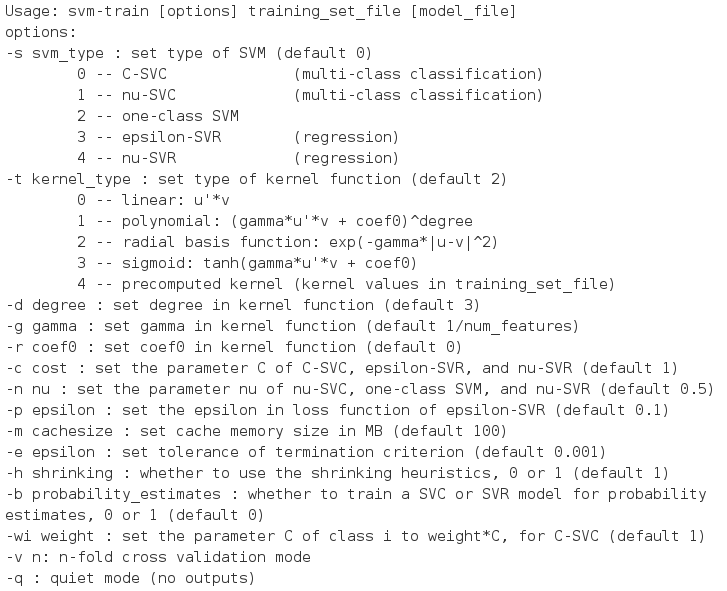
\includegraphics[width=0.8\linewidth]{figures/svmtrain.png}
	\end{enumerate}
\end{frame}

\begin{frame}{LibSVM-Matlab/Octave}
	Function options:
	\begin{enumerate}
		\item<0>\vspace{-0.25in}
		\item \textcolor{red}{svmpredict()} \\
		\url{https://raw.github.com/cjlin1/libsvm/master/README}\\
			Usage: svm-predict [options] test\_file model\_file output\_file
options:
-b probability\_estimates: whether to predict probability estimates, 0 or 1 (default 0); for one-class SVM only 0 is supported
	\end{enumerate}
\end{frame}

\begin{frame}[fragile]
\scriptsize
\begin{lstlisting}[language=Matlab]
% read provided data heart\_scale
[heart_label, heart_data] = libsvmread('../heart_scale');

% SVM training 
model = svmtrain(heart_label, heart_data, '-c 1 -g 0.07');

% test the training data
[predict_label, accuracy, dec_values] ...
= svmpredict(heart_label, heart_data, model); 
\end{lstlisting}
\normalsize
\end{frame}

\begin{frame}{LibSVM-Python}
	Setup:
	\begin{enumerate}
	\item Environment: Python, C/C++ compiler (MSVS in Windows or gcc in Linux/Unix).
	\item Build binaries\\
		Type \textit{make} in terminal if in Linux/Unix, copy ../windows/libsvm.dll to C:/WINDOWS/system32/ if in Windows.
	\item Use other python interface of LibSVM like scikit-learn \url{http://scikit-learn.org/stable/modules/svm.html}
	\end{enumerate}
\end{frame}

\begin{frame}[fragile]
Quick start: 
\scriptsize
\begin{lstlisting}[language=Python]
# import libsvm packages 
>>> from svmutil import *

# Read data in LIBSVM format
>>> y, x = svm_read_problem('../heart_scale')

# SVM training
>>> m = svm_train(y[:200], x[:200], '-c 4')

# SVM testing
>>> p_label, p_acc, p_val = svm_predict(y[200:], x[200:], m)
\end{lstlisting}
\normalsize
\end{frame}

\end{document} 